% !TEX TS-program = pdfLaTeX
% !TEX encoding = UTF-8 Unicode

% Copyright 2010 by Pedro Furlanetto 
%
% In principle, this file can be redistributed and/or modified under
% the terms of the GNU Public License, version 2.

% Based on Till Tantau beamer template

\documentclass{beamer}
%\documentclass[draft]{beamer}

\mode<presentation>
{
  \usetheme{Warsaw}
  \setbeamercovered{transparent}
}

\usepackage[utf8]{inputenc}  % levar em consideração que é um arquivo em utf8
\usepackage{times}                 % um fonte que tenha acentos
\usepackage[T1]{fontenc}      % levando em consideração utf8 na hora de escolher as letras da fonte

\usepackage{hyperref}
\usepackage{graphicx}
\usepackage[english]{babel}
\usepackage{color}
\usepackage{listings}
 
% "define" Scala
\lstdefinelanguage{Scala}{
  morekeywords={abstract,case,catch,class,def,%
    do,else,extends,false,final,finally,%
    for,if,implicit,import,match,mixin,%
    new,null,object,override,package,%
    private,protected,requires,return,sealed,%
    super,this,throw,trait,true,try,%
    type,val,var,while,with,yield}, % scala>
  otherkeywords={=,:,=>,<-,<\%,<:,>:,\#,@},
  sensitive=true,
  morecomment=[l]{//},
  morecomment=[n]{/*}{*/},
  morestring=[b]",
  morestring=[b]',
  morestring=[b]""",
 % literate={=>}{$\Rightarrow$ }2 {<-}{$\leftarrow$}2 {->}{$\rightarrow$}2
}


\definecolor{dkgreen}{rgb}{0,0.6,0}
\definecolor{gray}{rgb}{0.5,0.5,0.5}
\definecolor{mauve}{rgb}{0.58,0,0.82}

% Default settings for code listings
\lstset{frame=tb,
  language=Scala,
  aboveskip=3mm,
  belowskip=3mm,
  showstringspaces=false,
  columns=flexible,
  basicstyle={\scriptsize\ttfamily},
  numbers=none,
  numberstyle=\tiny\color{gray},
  keywordstyle=\color{blue},
  commentstyle=\color{dkgreen},
  stringstyle=\color{mauve},
  frame=single,
  breaklines=true,
  breakatwhitespace=true,
  tabsize=3,
  mathescape=true,
  resetmargins=true,
  showtabs=true
}

\setbeamertemplate{navigation symbols}{}%remove navigation symbols

\title{Hacking Scaladoc}

%\subtitle{ \includegraphics[height=1cm]{lighting2.jpg}}

\author{Pedro Furlanetto}

\institute
{
  %Thanks Yuvi and Brian!\\
\begin{minipage}{0.6\textwidth}
\begin{flushleft} 
%includegraphics[height=1.5cm]{ideaisconf.png} 
\end{flushleft}
\end{minipage}
\begin{minipage}{0.3\textwidth}
%\centering{ \includegraphics[height=2cm]{ideais-grande.jpg}}
\end{minipage}
  
}

\date[Scalathon 2011] % (optional, should be abbreviation of conference name)
{Scalathon, 2011}

\subject{Hacking Scalathon}

%\logo{\includegraphics[height=1cm]{ideais-grande.jpg}}

\AtBeginSection[]
{
  \begin{frame}<beamer>{}
    \tableofcontents[currentsection,currentsubsection,sectionstyle=show/shaded,subsectionstyle=show/show/shaded]
  \end{frame}
}

%\beamerdefaultoverlayspecification{<+->}

\begin{document}

%\begin{frame}  
% 	%\centering{\includegraphics[height=1cm]{Scala_Logo2008.png}}
%	\titlepage
%\end{frame}

%\begin{frame}{Resumo}
%  \tableofcontents
%\end{frame}

\section{Overview}

\subsection{More than simple Html generator!}

\begin{frame}{More than simple Html generator}
	\begin{itemize} %[<+->]
	\item Generates a representation for
		\begin{itemize}  
		\item the Scala structures (traits, classes, vals etc)
		\item Documentation
		\item The wiki syntax
		\end{itemize}
	\item Attachable processors for these (almost there)
	\end{itemize}
\end{frame}

\subsection{Model for Documentation}
\begin{frame}{Model for Documentation} 
	scala.tools.nsc.doc.Entity.scala:
	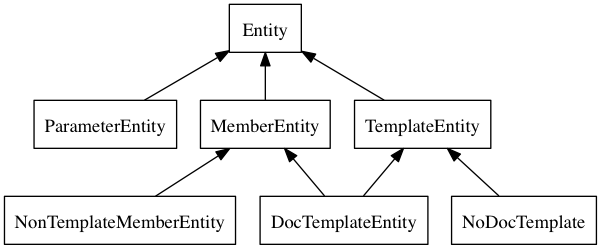
\includegraphics[width=11cm]{../docs/ScaladocModelDoc.png} %
\end{frame}


\subsection{Model for Scala}
\begin{frame}{Model for Scala}  
	scala.tools.nsc.doc.Entity.scala:
	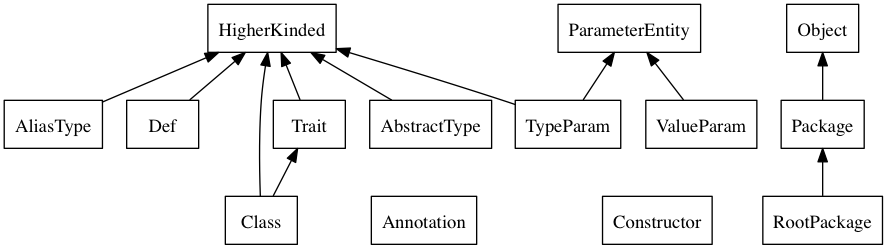
\includegraphics[width=11cm]{../docs/ScaladocModelScala.png} %
\end{frame}

\subsection{Model for Wiki}
\begin{frame}{Model for Wiki} 
	
\end{frame}

\subsection{Inner Workings}
\begin{frame}{Inner Workings} 
	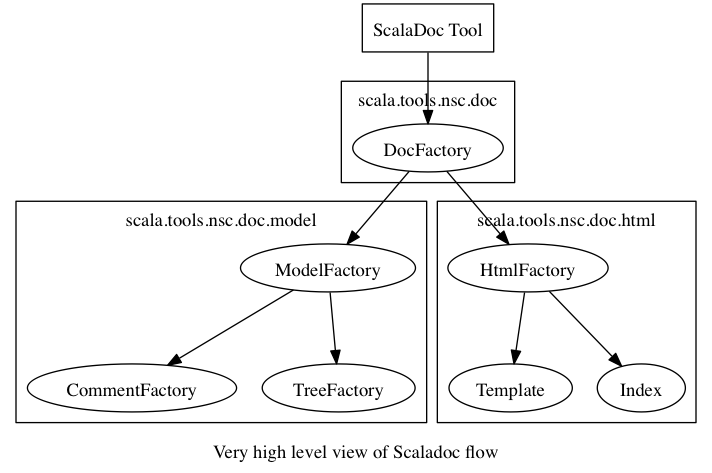
\includegraphics[width=11cm]{../docs/flow.png} 
\end{frame}

\section{How to Hacking it!}

\subsection{Enviroment}
\begin{frame}{Enviroment} 
	
\end{frame}

\subsection{Running}
\begin{frame}{Running} 
	
\end{frame}

\subsection{A little help}
\begin{frame}{A little help} 
	
\end{frame}

\subsection{Examples}
\begin{frame}{Examples} 
	
\end{frame}


\end{document}


